\section{Planarität testen}

\textbf{Problem}: Gegeben ein Graph $G$ als Adjazenzliste, entscheide ob $G$ planar ist

\textbf{Möglichkeit}: 
\begin{itemize}
	\item Teste auf $K_5$- oder $K_{3,3}$-Unterteilung
	\item Es existiert ein theoretisch effizienter, aber nicht praktikabler Algorithmus dafür, da die Laufzeit sehr groß werden kann
	\item Im Folgenden: \textbf{LR-Planarität}
\end{itemize}

\textbf{Annahmen}:
\begin{itemize}
	\item $G$ hat keine Mehrfachkante
	\item $G$ hat keine Schlingen
	\item $G$ hat keine Brücken, also liegt jede Kante auf einem Kreis
	\item $G$ ist zusammenhängend
\end{itemize}

\textbf{Vorbereitendes Vorgehen}:
\begin{itemize}
	\item Tiefensuche von beliebigem Startknoten
	\item Nummeriere Knoten in Explorierungsreihenfolge
	\item Orientiere Baumkanten in Explorierungsreihenfolge und Nichtbaumkanten vom Knoten mit größerer DFS-Zahl zum Knoten mit kleinerer DFS-Zahl
	\begin{center}
		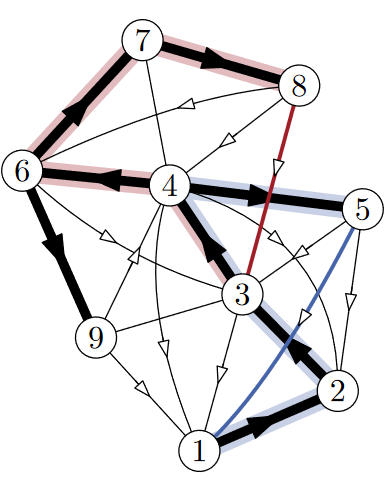
\includegraphics[width=0.2\textwidth]{images/dfs.png}
	\end{center}
\end{itemize}

\textbf{Erste Beobachtungen}:
\begin{itemize}
	\item Nichtbaumkanten verbinden immer zwei Knoten auf einem Wurzel-Blatt-Pfad.
	\item Jede Nichtbaumkante $e$ schließt einen eindeutigen Kreis mit den Baumkanten (\textbf{Fundamentalkreis} zu $e$).
	\item Jede planare Zeichnung von $G$ liefert auch eine planare Zeichnung des DFS-Baums. Betrachte Zeichnung mit der Wurzel an der äußeren Facette.
	\item Jede Nichtbaumkante $e$ führt entweder links (\textbf{$\mathbf{L}$-Kante}) oder rechts (\textbf{$\mathbf{R}$-Kante}) am Baum zurück.
	\item Um herauszufinden, ob $G$ planar ist, müssen wir entweder eine Einteilung der Nichtbaumkanten in $L$- und $R$-Kanten finden bei der keine Überschneidungen entstehen (\textbf{LR-Zerlegung}) oder zeigen, dass eine solche Einteilung nicht existiert.
\end{itemize}
\bigskip
\textbf{Definition}: Sei $e$ eine Kante. Eine Nichtbaumkante $(x, y)$ heißt \textbf{Rückkante} von $e$, wenn $e$ auf dem Fundamentalkreis von $(x, y)$ liegt. Dann nennt man $y$ einen \textbf{Rückkehrpunkt} von $e$. Ist $e$ eine Nichtbaumkante, so ist $e$ seine einzige und eigene Rückkante mit eindeutigem Rückkehrpunkt.
\begin{center}
	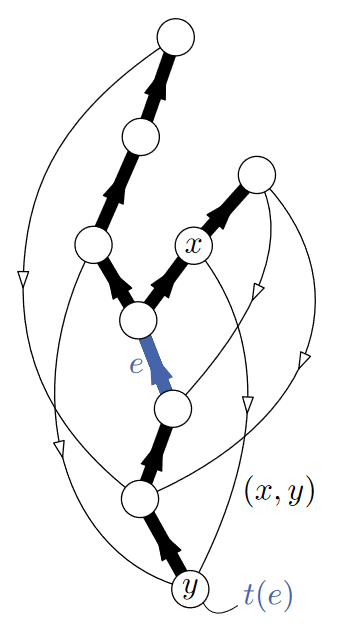
\includegraphics[width=0.2\textwidth]{images/back-edge.png}
\end{center}

\textbf{Definition}: Sei $e$ eine Kante. Der tiefste Rückkehrpunkt von $e$
$$t(e)\coloneqq \text{kleinste DFS-Zahl eines Rückkehrpunktes}$$ nennt man den \textbf{Tiefpunkt} von $e$.

\textbf{Definition}: Eine \textbf{Gabel} sind zwei Kanten mit dem gleichen Startpunkt, also $e_1=(u,v_1)$ und $e_2=(u,v_2)$.

\textbf{Definition}: Für eine Gabel $e_1=uv_1$, $e_2=uv_2$ definiere die Mengen
\begin{itemize}
	\item $R(e_1,e_2)\coloneqq\{e \text{ Rückkante von }e_1 \text{ mit }t(e_2)<t(e)<u\}$
	\item $R(e_2,e_1)\coloneqq\{e \text{ Rückkante von }e_2 \text{ mit }t(e_1)<t(e)<u\}$
\end{itemize} 
Zwei Kanten $f_1,f_2$ haben einen \textbf{Konflikt} bezüglich $e_1,e_2$, wenn
\begin{itemize}
	\item $f_1,f_2\in R(e_1,e_2)$ oder $f_1,f_2\in R(e_2,e_1)$ (\textbf{Gleichheitskonflikt})
	\item $f_1 \in R(e_1,e_2)$ und $f_2\in R(e_2,e_1)$ oder umgekehrt (\textbf{Ungleichheitskonflikt})
\end{itemize}
\begin{center}
	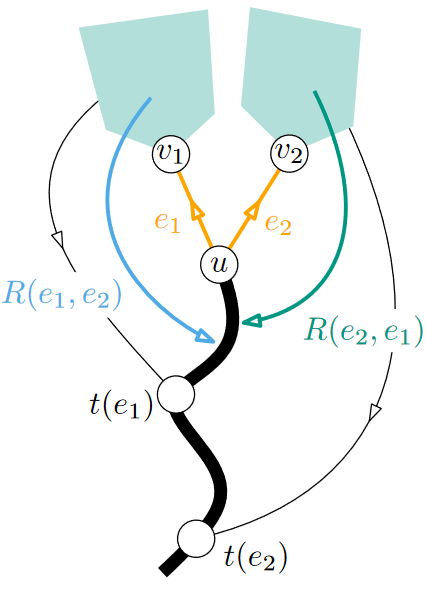
\includegraphics[width=0.25\textwidth]{images/konflikt.png}
\end{center}

\textbf{Definition}: Eine \textbf{LR-Zerlegung} ist eine Partition der Nichtbaumkanten in $L$ und $R$, sodass je zwei Kanten $f_1,f_2$
\begin{itemize}
	\item mit Gleichheitskonflikt in der gleichen Menge sind.
	\item mit Ungleichheitskonflikt in unterschiedlichen Mengen sind.
\end{itemize}
\bigskip
\textbf{Satz}: Folgende Aussagen sind äquivalent:
\begin{itemize}
	\item $G$ ist planar.
	\item Es gibt eine LR-Zerlegung bezüglich einer Tiefensuche.
	\item Es gibt zu jeder Tiefensuche eine LR-Zerlegung
\end{itemize}
\textit{Der Beweis des Satzes wird später skizziert}.\\

\textbf{Planaritätstest basierend auf LR-Zerlegung}
\begin{enumerate}
	\item Tiefensuche auf Graph in $\mathcal{O}(n)=\mathcal{O}(|V(G)|)$
	\item Bestimme naiv alle Kantenkonflikte in $\mathcal{O}(n^2)$, indem man sich z.B. alle Kantenpaare anschaut
	\item Baue Hilfsgraph $H$ mit
	\begin{itemize}
		\item Knoten in $H$ sind Kanten von $G$.
		\item Kanten in $H$ sind Ungleichheitskonflikte in $G$.
		\item Knoten in $H$ werden verschmolzen, wenn sie einen Gleichheitskonflikt haben.
	\end{itemize}
	\begin{center}
		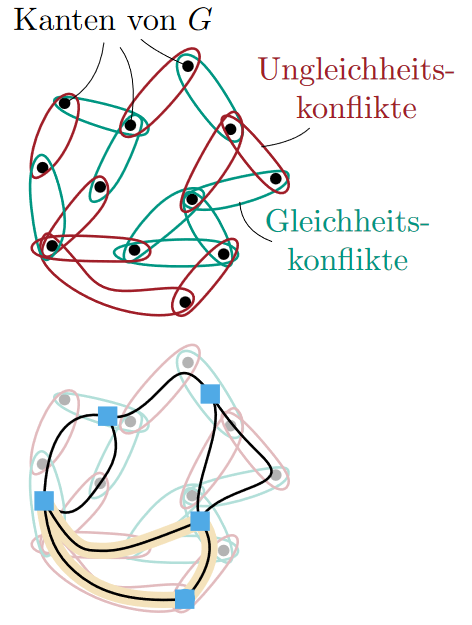
\includegraphics[width=0.25\textwidth]{images/planar-test.png}
	\end{center}
	\item LR-Zerlegung von $G$ existiert $\iff$ $H$ ist bipartit. Teste also den Graphen auf Bipartitheit. Das geht in $\mathcal{O}(n^2)$
\end{enumerate}
$\implies$ Damit haben wir einen Planaritätstest in $\mathcal{O}(n^2)$. Eine Beschleunigung auf $\mathcal{O}(n)$ ist aber möglich.\\

\textit{Korrektheitsbeweis vom obigen Satz}: